\section{L'Equazione Logistica}

L'equazione logistica è un modello matematico molto utile per descrivere una vasta gamma di fenomeni.

\subsection{Il Modello}

L'\textbf{equazione logistica} è un'equazione differenziale al prim'ordine a variabili separabili nella forma: 

\begin{equation}
	\dot{x}=x(1-x)
	\label{logequation}
\end{equation}

Dalla (\ref{logequation}) è immediato osservare che il suo comportamento è determinato da due fattori:

\begin{itemize}
	\item Crescita: dato da un termine lineare \\
	\item Decrescita: dato da un termine quadratico con coefficiente negativo \\
\end{itemize}

\paragraph{Una soluzione esplicita}

Infine è possibile ricavare una forma analitica della sua soluzione:

\begin{equation}
	x(t)=\frac{ce^t}{1+ce^t}
	\label{logfunction}
\end{equation}

\begin{center}
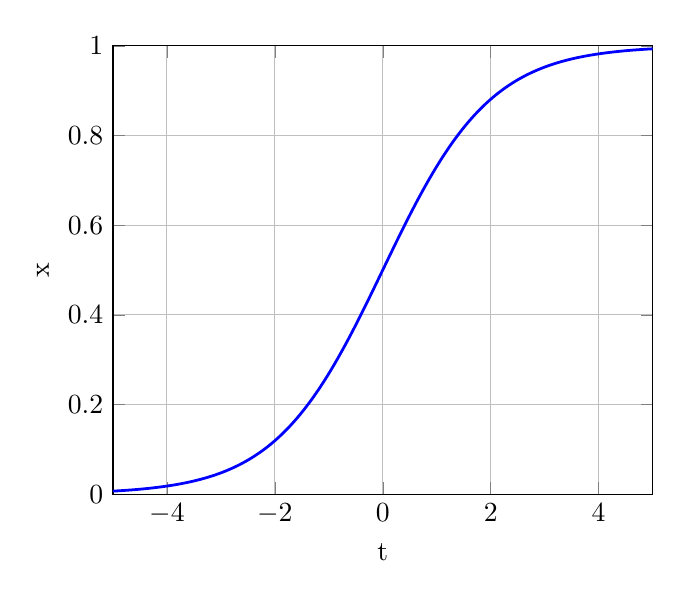
\begin{tikzpicture}
	\begin{axis}[xmin = -5, xmax = 5,
		ymin = 0, ymax = 1,
		grid, xlabel = t, ylabel = x,
		samples=500
		]
		\addplot[% opzioni di disegno
		color=blue, line width=1pt
		] {
			exp(x)/(1+exp(x)) % espressione matematica
		};
	\end{axis}
    \label{graph}
\end{tikzpicture}
\end{center}